\documentclass[./main.tex]{subfiles}
\graphicspath{{\subfix{./figs}}}

% ------------ main document ------------
\begin{document}
\nolinenumbers

% style setup
\newpage
\renewcommand{\headrulewidth}{0pt}
\thispagestyle{fancy}
%... then configure it
\fancyhf{} % Clear all header and footer fields.
\fancyfoot{} % clear all footer fields
\fancyfoot[C]{\thepage}

\par \hfill
\vspace{40mm}
\begin{adjustwidth}{45pt}{45pt}
\begin{center}
    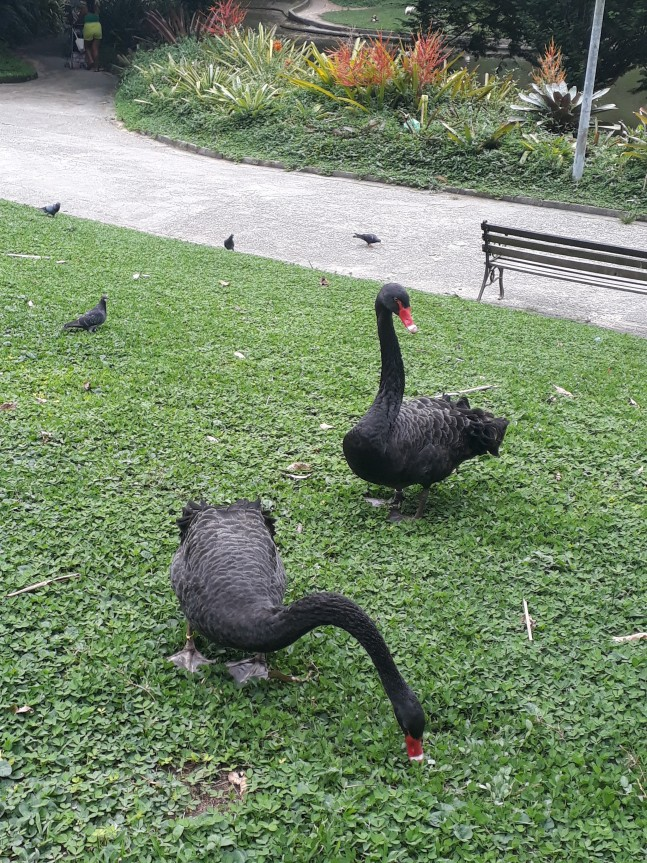
\includegraphics[scale=1]{fig_swan.jpg}\\
\end{center}
\vspace{10mm}
\noindent \textsf{Em 16 de Fevereiro de 2023, às 15 horas e 23 minutos, dois cisnes pretos foram observados no parque aos fundos do Palácio das Laranjeiras, Rio de Janeiro, Brasil. Um único cisne preto já seria suficiente para provar que \textit{nem todos os cisnes são brancos}.}
\end{adjustwidth}
\clearpage
\end{document}